\documentclass[handout]{beamer}

% math packages
\usepackage{amssymb}

% theme
\usetheme{Rochester}
\usecolortheme{dove}
\usefonttheme{default}

% make the title BIG
\setbeamerfont{title}{series=\bfseries,size=\Huge, parent=structure}

% remove the side title header
\setbeamertemplate{headline}{}

%gets rid of bottom navigation bars
\setbeamertemplate{footline}{}

%gets rid of navigation symbols
\setbeamertemplate{navigation symbols}{}

% define "head" commands for transitions
\newcommand{\headone}{\centering \bf \Huge}
\newcommand{\headtwo}{\centering \bf \LARGE}
\newcommand{\headthree}{\centering \bf \Large}

% define a "spaceit" command for spacing between paragraphs
\newcommand{\spaceit}{\vspace{10mm}}

% define a "red" command to make text red.
\newcommand{\red}[1]{\textcolor{red}{#1}}

% simply the style of the lists
\setbeamertemplate{itemize items}[default]
\setbeamertemplate{enumerate items}[default]

% increase the default spacing between equations
\setlength{\jot}{5pt}

% custom color for "blockcode"
\usepackage{fancyvrb,color}

\DefineVerbatimEnvironment{blockcode}
  {Verbatim}
  {formatcom=\color{blue}}


\begin{document}
\title{An Introduction to Maximum Likelihood Estimation}   
\author{Carlisle Rainey} 
\date{} % remove date 

\frame{\titlepage} 

\frame{
\textbf{A maximum likelihood estimator selects the parameter vector $\theta$ that maximizes the probability of the observed data $y$ across the parameter space $\Theta$.}\\\vspace{5mm}

\pause Under which $\theta$ would these data most likely occur?\\\vspace{5mm}

\begin{itemize}
\pause \item Assumes that the model $Y \sim f(y | \theta)$ is correct.
\pause \item Optimal asymptotic properties.
\pause \item Usually reasonable in small samples.
\pause \item Intuitive appeal and usually easy to implement.
\end{itemize}
}

\frame{
Once we know (or assume) the probability model $Y \sim f(y | \theta)$, deriving an estimator is easy--we just use maximum likelihood.\spaceit

\footnotesize{
\pause General Process of Maximum Likelihood Estimation
\begin{enumerate}
\pause \item Calculate the probability of the data given the parameters. This is the ``likelihood function,'' which we might write this as $p(y | \theta)$ or $\mathcal{L}(\theta | y)$. We typically use $\mathcal{L}(\theta | y)$ since we're going to maximize across $\theta$, but the two are equal.
\pause \item Take the log and remove as many powers and products as possible. This gives us the ``log-likelihood function,'' which  write as $\log\mathcal{L}(\theta | y)$. In addition to logging, we can apply any monotonic \textit{increasing} function we like to $\mathcal{L}$ (i.e., drop constants). We apply these transformation because it make the maximization easier but preserves the maximum.
\pause \item Use calculus to find the maximum of the log-likelihood function. $\underset{\theta}{\arg\max \mathcal{L}(y | \theta)}$. Sometimes this will be difficult or impossible and we'll use a hill-climbing algorithm (i.e., numerical optimization).
\end{enumerate}
}}

\frame{ 
\headone
Binomial Example
}

\frame{
Start with the probability model $Y \sim f(y | \theta)$, which in the case of the binomial model is $Y \sim \text{binomial}(y | n, \pi)$.
\spaceit

\pause Questions:
\begin{enumerate}
\pause \item What is the \textit{support} of the binomial distribution? \pause \red{$y \in \{0, 1, 2, ..., n\}$.}
\pause \item Is $y$ a discrete random variable or a continuous random variable? \pause \red{Discrete.}
\pause \item What is the pdf/pmf? \pause \red{$f(y | n, \pi) = \displaystyle{n \choose y}\pi^y(1 - \pi)^{n - y}$.}
\end{enumerate}
}

\frame{
Step 1: Write down the likelihood function.
\begin{equation}\nonumber
\pause \mathcal{L}(\pi | y, n) = p(y | n, \pi) = \displaystyle{n \choose y}\pi^y(1 - \pi)^{n - y}
\end{equation}
\pause In this case, it's just the pmf, but that will not always be the case. This will be harder when we get multiple observations.
}

\frame{
Step 2: Take the log and reduce.
\begin{equation*}
\begin{aligned}
\pause \mathcal{L}(\pi | y, n) &= \displaystyle{n \choose y}\pi^y(1 - \pi)^{n - y}\\
\pause \log \mathcal{L}(\pi | y, n) &= \log\left[ \displaystyle{n \choose y}\pi^y(1 - \pi)^{n - y} \right]\\
\pause &= \log\displaystyle{n \choose y} + \log\left[\pi^y \right] + \log \left[ (1 - \pi)^{n - y} \right]\\
\pause &\propto \log\left[\pi^y \right] + \log \left[ (1 - \pi)^{n - y} \right]\\
\pause \log\mathcal{L}(\pi | y, n) &\propto y \log\pi+ (n - y) \log(1 - \pi)
\end{aligned}
\end{equation*}
}

\frame{
\headtwo
Step 3: Maximize.\\
\vspace{10mm}
Analytical Optimization
}

\frame{
Start with the log-likelihood and take the derivative with respect to the parameter.
\begin{small}
\begin{equation*}
\begin{aligned}
\pause \log\mathcal{L}(\pi | y, n) &\propto y \log\pi+ (n - y) \log(1 - \pi)\\
\pause \dfrac{\partial \mathcal{L}(\pi | y, n)}{\partial \pi} &\propto \dfrac{\partial}{\partial \pi} \left[y \log\pi+ (n - y) \log(1 - \pi)\right]\\
\pause &\propto \dfrac{\partial}{\partial \pi} \left[y \log\pi\right] + \dfrac{\partial}{\partial \pi} \left[(n - y) \log(1 - \pi)\right]\\
\pause &\propto y \dfrac{\partial}{\partial \pi} \left[\log\pi\right] + (n - y)  \dfrac{\partial}{\partial \pi} \left[\log(1 - \pi)\right]\\
\pause &\propto y \left(\dfrac{1}{\pi}\right) + (n - y)  \dfrac{\partial}{\partial \pi} \left[\log(1 - \pi)\right]\\
\pause &\propto y \left(\dfrac{1}{\pi}\right) + (n - y) \left[\dfrac{1}{1 - \pi}\right](-1)\\
\pause \dfrac{\partial \mathcal{L}(\pi | y, n)}{\partial \pi} &\propto \dfrac{y}{\pi} - \dfrac{n - y}{1 - \pi}
\end{aligned}
\end{equation*}
\end{small}
}

\frame{
Now we'll set the derivative equal to zero to find the spot where the log-likelihood is flat. That will be our estimate $\hat{\pi}$.
\begin{small}
\begin{equation*}
\begin{aligned}
\pause \dfrac{y}{\hat{\pi}} - \dfrac{n - y}{1 - \hat{\pi}} &= 0\\
\pause \dfrac{(1 - \hat{\pi})y}{\hat{\pi}(1 - \hat{\pi})} - \dfrac{\hat{\pi}(n - y)}{\hat{\pi}(1 - \hat{\pi})} &= 0\\
\pause (1 - \hat{\pi})y - \hat{\pi}(n - y) &= 0\\
\pause y - \hat{\pi} y - (\hat{\pi} n - \hat{\pi} y) &= 0\\
\pause y - \hat{\pi} y - \hat{\pi} n + \hat{\pi} y &= 0\\
\pause y - \hat{\pi}n &= 0\\
\pause y &= \hat{\pi} n \\
\pause \dfrac{y}{n} &= \hat{\pi}
\end{aligned}
\end{equation*}
\end{small}
}

\frame{
Comment: Strictly speaking, we should show that the second-derivative is negative at $\hat{\pi}$. However, we'll rarely encounter situations in which this is \textit{not} the case.
}

\frame{
\headtwo
Numerical Optimization
}

\frame{
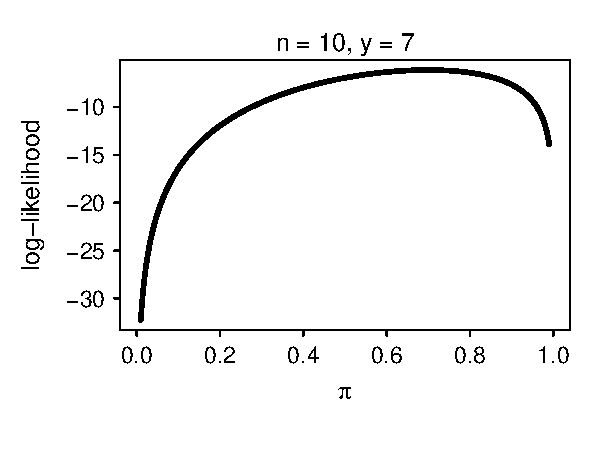
\includegraphics[scale = 1.1]{figs/ll-binom-10-7.pdf}
}

\frame{
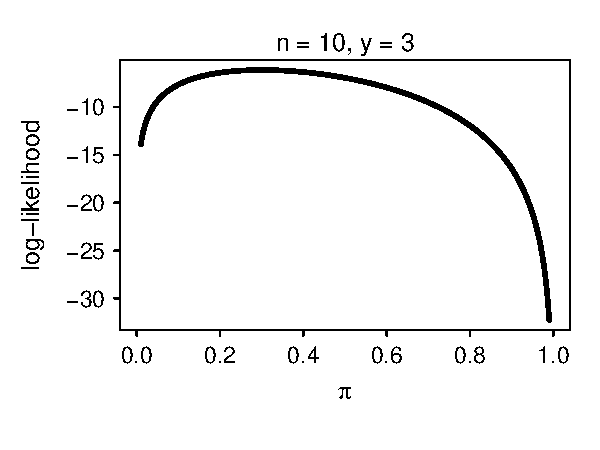
\includegraphics[scale = 1.1]{figs/ll-binom-10-3.pdf}
}

\frame{
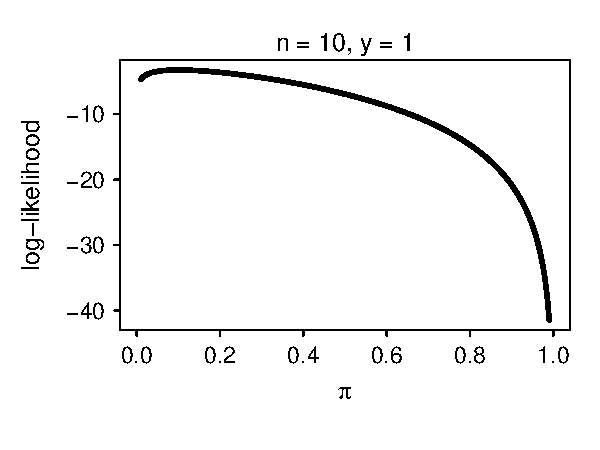
\includegraphics[scale = 1.1]{figs/ll-binom-10-1.pdf}
}

\frame{
\headthree
Hill-Climbing Algorithms
}

\frame{
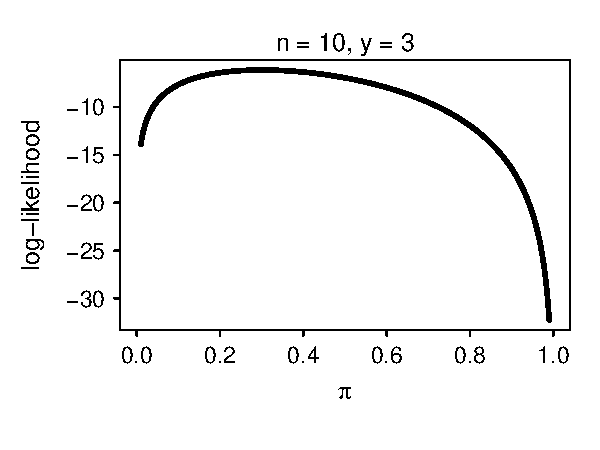
\includegraphics[scale = 1.1]{figs/ll-binom-10-3.pdf}
}

\begin{frame}[fragile]
Numerical Optimization in R \spaceit

\begin{enumerate}
\item Create the log-likelihood function as a function in R.
\pause \begin{blockcode} 
ll.fn.dist <- function(theta, y) {
  ...
}
\end{blockcode}
\pause \item Use \texttt{optim()} to find the maximum of the function.
\pause \begin{blockcode}
est <- optim(par = c(...), fn = ll.fn.dist, ...,
                    control = list(fnscale = -1))
\end{blockcode}
\end{enumerate}
\end{frame}

\begin{frame}[fragile]
The computation for the binomial case.
\pause \begin{blockcode} 
# log-likelihood for binomial
ll.fn.binom <- function(p, n, y) {
  y*log(p) + (n - y)*log(1 - p)
}
\end{blockcode}

\pause \begin{blockcode}
# data
y <- 7
n <- 10
\end{blockcode}

\pause \begin{blockcode}
# optimize
est <- optim(par = .5, fn = ll.fn.binom, y = y, n = n,
             control = list(fnscale = -1),
             method = "Brent",  # for 1d problems
             lower = 0, upper = 1)  # req for Brent
\end{blockcode}
\end{frame}

\begin{frame}[fragile]
The results of the \texttt{optim()} call.
\begin{blockcode} 
> est
$par
[1] 0.7

$value
[1] -6.108643

$counts
function gradient 
      NA       NA 

$convergence
[1] 0

$message
NULL
\end{blockcode}
\end{frame}

\begin{frame}[fragile]
We could even write a function to handle this automatically.
\begin{small}
\pause \begin{blockcode} 
# function to estimate binomial model
est.binom <- function(y, n) {
  est <- optim(par = .5, fn = ll.fn.binom, y = y, n = n,
            control = list(fnscale = -1),
            method = "Brent",  # for 1d problems
            lower = 0, upper = 1)
  if (est$convergence != 0) print("Model did not converge!")
  res <- list(est = est$par)
  return(res)
}
\end{blockcode}

\pause \begin{blockcode}
# estimate binomial model
m1 <- est.binom(7, 10)
\end{blockcode}
\end{small}
\end{frame}

\frame{
\textbf{Maximum Likelihood Estimation}
\begin{enumerate}
\pause \item Write down a probability model.
\pause \item Find the probability of the data given the parameters--the likelihood function.
\pause \item Take the log and simplify.
\pause \item Maximize.
	\begin{itemize}
	\pause \item Analytically. (Usually difficult or impossible.)
	\pause \item Numerically. (Usually easier.)
	\end{itemize}
\end{enumerate}
}

\frame{
\headone
Normal Example\\
\normalsize{(Adding multiple observations.)}
}

\frame{
Start with the probability model $Y_i \sim f(y_i | \theta)$, which in the case of the ``stylized'' normal model is $Y_i \sim N(y_i | \mu, 1)$. \pause We're assuming a known variance so that we have just one parameter to estimate. \pause However, we're going to assume that we have multiple observations, so that $y = [y_1, y_2, ,..., y_n]$.
\spaceit

\pause Questions:
\begin{enumerate}
\pause \item What is the \textit{support} of the normal distribution? \pause \red{The real line.}
\pause \item Is $y$ a discrete random variable or a continuous random variable? \pause \red{Continuous.}
\pause \item What is the pdf/pmf? \pause \red{$f(y_i | \mu, \sigma) = \dfrac{1}{\sigma \sqrt{2\pi}}e^{-\dfrac{(y_i - \mu)^2}{2\sigma^2}}$.}
\end{enumerate}
}

\frame{
Step 1: Write down the likelihood function. \pause Recall that we can obtain the probability of $y_1$ AND $y_2$ AND ... AND $y_n$ by multiplying the probabilities of each (assuming independence).
\begin{equation}\nonumber
\pause \mathcal{L}(\mu | y ) = \displaystyle\prod_{i = 1}^n \overbrace{p(y_i | \mu)}^{density} = \displaystyle\prod_{i = 1}^n \dfrac{1}{\sqrt{2\pi}}e^{-\dfrac{(y_i - \mu)^2}{2}}
\end{equation}
\pause When you have multiple observations (as is usually the case), you'll get a product like this.
}

\frame{
Step 2: Take the log and reduce.
\begin{scriptsize}
\begin{equation*}
\begin{aligned}
\pause \mathcal{L}(\mu | y) &= \displaystyle\prod_{i = 1}^n \dfrac{1}{\sqrt{2\pi}}e^{-\dfrac{(y_i - \mu)^2}{2}}\\
\pause \log \mathcal{L}(\mu | y) &= \log \displaystyle\prod_{i = 1}^n \dfrac{1}{\sqrt{2\pi}}e^{-\dfrac{(y_i - \mu)^2}{2}}\\
\pause &= \displaystyle \sum_{i = 1}^n \log \dfrac{1}{\sqrt{2\pi}}e^{-\dfrac{(y_i - \mu)^2}{2}}\\
\pause &= \displaystyle \sum_{i = 1}^n \left[\overbrace{\log \dfrac{1}{\sqrt{2\pi}}}^{constant} + \log e^{-\dfrac{(y_i - \mu)^2}{2}}\right]\\
\pause &\propto \displaystyle -\sum_{i = 1}^n \dfrac{(y_i - \mu)^2}{2}\\
\pause \log \mathcal{L}(\mu | y) &\propto \displaystyle -\sum_{i = 1}^n (y_i - \mu)^2~~\pause\text{\color{purple}{Look familiar?}}
\end{aligned}
\end{equation*}
\end{scriptsize}
}

\frame{
\textbf{Step 3: Maximize.}\vspace{3mm}

First, let's do a little rewriting.
\begin{scriptsize}
\begin{equation*}
\begin{aligned}
\pause \log \mathcal{L}(\mu | y) &= \displaystyle -\sum_{i = 1}^n (y_i - \mu)^2 \\
\pause &= \displaystyle -\sum_{i = 1}^n (y_i^2 - 2y_i\mu + \mu^2)\\
\pause &= -\left[ \displaystyle \sum_{i = 1}^n y_i^2 - \displaystyle \sum_{i = 1}^n 2y_i\mu + \displaystyle \sum_{i = 1}^n \mu^2 \right]\\
\pause &\propto -\left[- \displaystyle \sum_{i = 1}^n 2y_i\mu + \displaystyle \sum_{i = 1}^n \mu^2 \right]\\
\pause &\propto \displaystyle \sum_{i = 1}^n 2y_i\mu - \displaystyle \sum_{i = 1}^n \mu^2 \\
\pause \log \mathcal{L}(\mu | y) &\propto 2  \mu \displaystyle \sum_{i = 1}^n y_i - n\mu^2\
\end{aligned}
\end{equation*}
\end{scriptsize}
}

\frame{
\textbf{Step 3: Maximize.}\vspace{3mm}

Now, let's find the derivative
\begin{scriptsize}
\begin{equation*}
\begin{aligned}
\log \mathcal{L}(\mu | y) &\propto 2  \mu \displaystyle \sum_{i = 1}^n y_i - n\mu^2\\
\dfrac{\partial \log \mathcal{L}(\mu | y)}{\partial \mu} &\propto \dfrac{\partial}{\partial \mu} \left[2\mu \displaystyle \sum_{i = 1}^n y_i\right] - \dfrac{\partial}{\partial \mu}\left[n\mu^2\right]\\
\dfrac{\partial \log \mathcal{L}(\mu | y)}{\partial \mu} &\propto 2\displaystyle \sum_{i = 1}^n y_i - 2n\mu\\
\end{aligned}
\end{equation*}
\end{scriptsize}
}

\frame{
\textbf{Step 3: Maximize.}\vspace{3mm}

Now, let's set the derivative equal to zero and solve for $\hat{\mu}$.
\begin{equation*}
\begin{aligned}
\log \mathcal{L}(\hat{\mu} | y) \propto 2\displaystyle \sum_{i = 1}^n y_i - 2n\hat{\mu} &= 0\\
2\displaystyle \sum_{i = 1}^n y_i = 2n\hat{\mu}\\
\displaystyle \sum_{i = 1}^n y_i = n\hat{\mu}\\
\displaystyle \dfrac{\sum_{i = 1}^n y_i}{n} = \hat{\mu}\\
\end{aligned}
\end{equation*}
}

\begin{frame}[fragile]
Or we could write a little R function to do the optimization numerically.
\begin{scriptsize}
\pause \begin{blockcode} 
# log-likelihood for normal
ll.fn.norm <- function(mu, y) {
  -sum((y - mu)^2)
}
\end{blockcode}

\pause \begin{blockcode}
# function to estimate normal model
est.norm <- function(y) {
  est <- optim(par = 0, fn = ll.fn.norm, y = y,
               control = list(fnscale = -1),
               method = "Brent",  # for 1d problems
               lower = -100, upper = 100)
  if (est$convergence != 0) print("Model did not converge!")
  res <- list(est = est$par)
  return(res)
}
\end{blockcode}

\pause \begin{blockcode}
# data
y <- c(1.2, 3, 4.2)
\end{blockcode}

\pause \begin{blockcode}
# estimate mean
m1 <- est.norm(y)
\end{blockcode}
\end{scriptsize}
\end{frame}

\begin{frame}[fragile]
Now let's try a little fake data simulation.
\pause \begin{blockcode}
# set an unknown, but fixed, parameter mu
mu <- runif(1, -10, 10)
\end{blockcode}

\pause \begin{blockcode}
# simulate the data
y <- rnorm(1000, mu, 1)
\end{blockcode}

\pause \begin{blockcode}
# estimate mean
m1 <- est.norm(y)
\end{blockcode}
\end{frame}

\frame{
\textbf{Maximum Likelihood Estimation}
\begin{enumerate}
\pause \item Write down a probability model.
\pause \item Find the probability of the data given the parameters--the likelihood function.
\pause \item Take the log and simplify.
\item Maximize.
	\begin{itemize}
	\pause \item Analytically. (Usually difficult or impossible.)
	\pause \item Numerically. (Usually easier.)
	\end{itemize}
\end{enumerate}
}

\frame{
\headone
Beta Example\\
\normalsize{(Adding multiple parameters and an intractable log-likelihood.)}
}

\frame{
Start with the probability model $Y_i \sim f(y_i | \theta)$, which in the case of the beta model is $Y_i \sim \text{beta}(y_i | \alpha, \beta)$. \pause We now have two parameters to estimate and we're going to assume that we have multiple observations, so that $y = [y_1, y_2, ,..., y_n]$.
\spaceit

\pause Questions:
\begin{enumerate}
\pause \item What is the \textit{support} of the beta distribution? \pause \red{$[0, 1]$}
\pause \item Is $y$ a discrete random variable or a continuous random variable? \pause \red{Continuous.}
\pause \item What is the pdf/pmf? \pause \red{$f(y_i | \alpha, \beta) = \dfrac{y_i^{\alpha - 1}(1 - y_i)^{\beta - 1}}{B(\alpha, \beta)}$, where $B(\alpha, \beta) = \displaystyle \int_0^1 t^{\alpha - 1}(1 - t)^{\beta - 1}dt$ = \color{blue}{\texttt{beta(a, b)}}.}
\end{enumerate}
}

\frame{
Step 1: Write down the likelihood function. \pause Recall that we can obtain the probability of $y_1$ AND $y_2$ AND ... AND $y_n$ by multiplying the probabilities of each (assuming independence).
\begin{equation}\nonumber
\pause \mathcal{L}(\alpha, \beta | y ) = \displaystyle\prod_{i = 1}^n \overbrace{p(y_i | \alpha, \beta)}^{density} = \displaystyle\prod_{i = 1}^n \dfrac{y_i^{\alpha - 1}(1 - y_i)^{\beta - 1}}{B(\alpha, \beta)}
\end{equation}
\pause We see again, as will be usual, that we have this complicated product that will make our lives difficult.
}

\frame{
Step 2: Take the log and reduce.
\begin{scriptsize}
\begin{equation*}
\begin{aligned}
\pause \mathcal{L}(\alpha, \beta | y ) &= \displaystyle\prod_{i = 1}^n \dfrac{y_i^{\alpha - 1}(1 - y_i)^{\beta - 1}}{B(\alpha, \beta)}\\
\pause \log \mathcal{L}(\alpha, \beta | y ) &= \displaystyle\sum_{i = 1}^n \log \dfrac{y_i^{\alpha - 1}(1 - y_i)^{\beta - 1}}{B(\alpha, \beta)}\\
\pause &= \displaystyle\sum_{i = 1}^n \left[ \log y_i^{\alpha - 1} + \log (1 - y_i)^{\beta - 1} - \log B(\alpha, \beta)\right]\\
\pause &= \displaystyle\sum_{i = 1}^n \left[ (\alpha - 1)\log y_i + (\beta - 1)\log (1 - y_i) - \log B(\alpha, \beta)\right]\\
\pause &= \displaystyle\sum_{i = 1}^n \left[ (\alpha - 1)\log y_i + (\beta - 1)\log (1 - y_i)\right] - n \log B(\alpha, \beta)\\
&= (\alpha - 1) \sum_{i = 1}^n \log y_i + (\beta - 1) \sum_{i = 1}^n \log (1 - y_i) - n \log B(\alpha, \beta)\\
\pause \log \mathcal{L}(\alpha, \beta | y )&\propto \alpha \sum_{i = 1}^n \log y_i + \beta \sum_{i = 1}^n \log (1 - y_i) - n \log B(\alpha, \beta)
\end{aligned}
\end{equation*}
\end{scriptsize}
}

\frame{
\textbf{Step 3: Maximize}

If we wanted, we could work on this one analytically. (A homework problem requires this.)
\begin{enumerate}
\item Take the derivative w.r.t. $\alpha$.
\item Take the derivative w.r.t. $\beta$.
\item Set both equal to zero and solve. (Two equations and two unknowns.)
\end{enumerate}
But the last term $B(\alpha, \beta) = \int_0^1 t^{\alpha - 1}(1 - t)^{\beta - 1}dt$ is tricky!\\
\vspace{5mm}
So let's do it numerically.
}

\begin{frame}[fragile]
Let's just write a little R function to do the optimization numerically.
\begin{scriptsize}
\pause \begin{blockcode} 
# log-likelihood for beta
ll.fn.beta <- function(theta, y) {
  alpha <- theta[1]  # optim() requires a single parameter vector
  beta <- theta[2]
  ll <- alpha*sum(log(y)) + beta*sum(log(1 - y)) - 
           length(y)*log(beta(alpha, beta))
  return(ll)
}
\end{blockcode}

\pause \begin{blockcode}
# function to estimate beta model
est.beta <- function(y) {
  est <- optim(par = c(1, 1), fn = ll.fn.beta, y = y,
               control = list(fnscale = -1),
               method = "Nelder-Mead") # for >1d problems
  if (est$convergence != 0) print("Model did not converge!")
  res <- list(est = est$par)
  return(res)
}
\end{blockcode}

\pause \begin{blockcode}
# data
y <- c(0.5, 0.6, 0.7)

# estimate the shape parameters
m1 <- est.beta(y)
\end{blockcode}
\end{scriptsize}
\end{frame}

\begin{frame}[fragile]
Now let's try a little fake data simulation. This becomes more important now because it let's us test whether our function is working or not.
\pause \begin{blockcode}
# set unknown, but fixed, parameters alpha and beta
alpha <- runif(1, 0, 10)
beta <- runif(1, 0, 10)
\end{blockcode}

\pause \begin{blockcode}
# simulate the data
y <- rbeta(1000, alpha, beta)
\end{blockcode}

\pause \begin{blockcode}
# estimate shape parameters
m1 <- est.beta(y)
\end{blockcode}
\end{frame}

\frame{
\textbf{Maximum Likelihood Estimation}
\begin{enumerate}
\pause \item Write down a probability model.
\pause \item Find the probability of the data given the parameters--the likelihood function.
\pause \item Take the log and simplify.
\pause \item Maximize.
	\begin{itemize}
	\pause \item Analytically. (Usually difficult or impossible.)
	\pause \item Numerically. (Usually easier.)
	\end{itemize}
\end{enumerate}
}

\frame{
\begin{center}
\textbf{\Huge Remaining Questions}\\\vspace{10mm}
\pause How do we estimate the standard errors of our coefficient estimates?\\\vspace{10mm}
\pause How do we incorporate covariates into the model?
\end{center}
}


\end{document}
